\documentclass{report}
\usepackage[spanish]{babel}
\usepackage[utf8]{inputenc}
\usepackage{graphicx, longtable, float, titlesec, hyperref, xcolor}

\hypersetup{
    hidelinks = true
}

\titleformat{\chapter}[display]
  {\normalfont\bfseries}{}{0pt}{\Huge}

\begin{document}
    \begin{titlepage}
        \centering
        
\includegraphics[width=0.6\textwidth]{./img/miscelanio/logo.jpg}\\
        \vspace{1cm}
        \LARGE Sistemas de Gestión de Seguridad de Sistemas de Información\\
        \vspace{0.5cm}
        \Large Ingeniería Informática de Gestión y Sistemas de Información\\
        \vspace{3cm}
        \Huge Sistema Web\\
        \vspace{2.5cm}
        \Large Autores:\\
        \vspace{0.2cm}
        \large Xabier Gabiña\\
        \large Ainhize Martinez\\
        \large Marcos Martín\\
        \vfill
        \today
    \end{titlepage}
    \tableofcontents
    \chapter{Introducción}
    \chapter{Vulnerabilidades}
        \section{Rotura de control de acceso}
            \subsection{Acceso mediante URL}

            \clearpage
        \section{Fallos criptográficos}
            \subsection{Sniffing}
            \clearpage
            \subsection{MITM}
            \clearpage
        \section{Inyecciones}
            \subsection{SQL Injection}
                La primera vulnerabilidad que vamos a probar es la de SQL Injection con la intencion de obtener información de la base de datos.
                Para el analisis de esta vulnerabilidad vamos a utilizar la herramienta sqlmap. 
                Esta herramienta nos permite analizar una url y comprobar si es vulnerable a SQL Injection de forma sencilla y automatizada.
                En caso de querer usarla, se puede instalar con el siguiente comando:
                \begin{center}
                    \texttt{sudo apt-get install sqlmap}
                \end{center}
                Una vez instalada, hemos ejecutado el siguiente comando para realizar las pruebas:\\
                \begin{center}
                    \texttt{sqlmap -u http://localhost:81/login.php --wizard}
                \end{center}
                Este analisis nos ha dado como resultado que la url es vulnerable a 3 tipos de SQL Injection:
                \begin{itemize}
                    \item Boolean-based blind SQL injection
                    \item Error-based SQL injection
                    \item Time-based blind SQL injection
                \end{itemize}
                \begin{figure}[H]
                    \centering
                    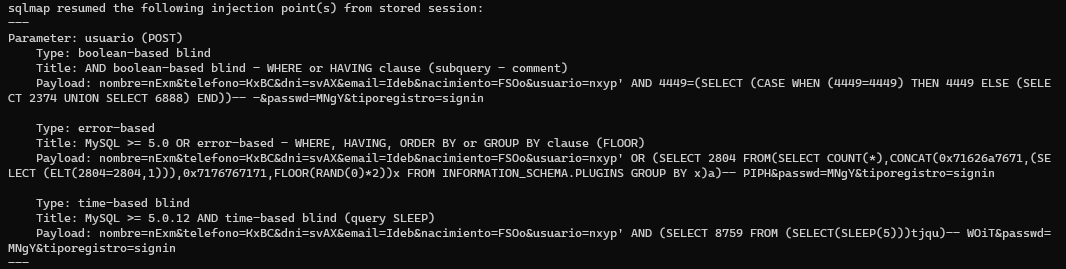
\includegraphics[width=1\textwidth]{./img/vulnerabilidades/2.3/1.1.png}
                    \caption{Puntos de injección}
                \end{figure}
                \clearpage
                Y es mediante el uso de estas vulnerabilidades que sqlmap, automaticamente, ha conseguido obtener las dos tablas de la base de datos:
                \begin{figure}[H]
                    \centering
                    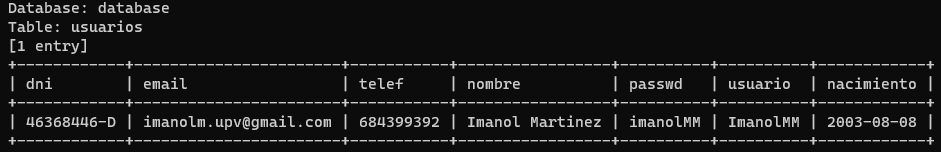
\includegraphics[width=1\textwidth]{./img/vulnerabilidades/2.3/1.2.png}
                    \caption{Tabla usuarios de la base de datos}
                \end{figure}
                \begin{figure}[H]
                    \centering
                    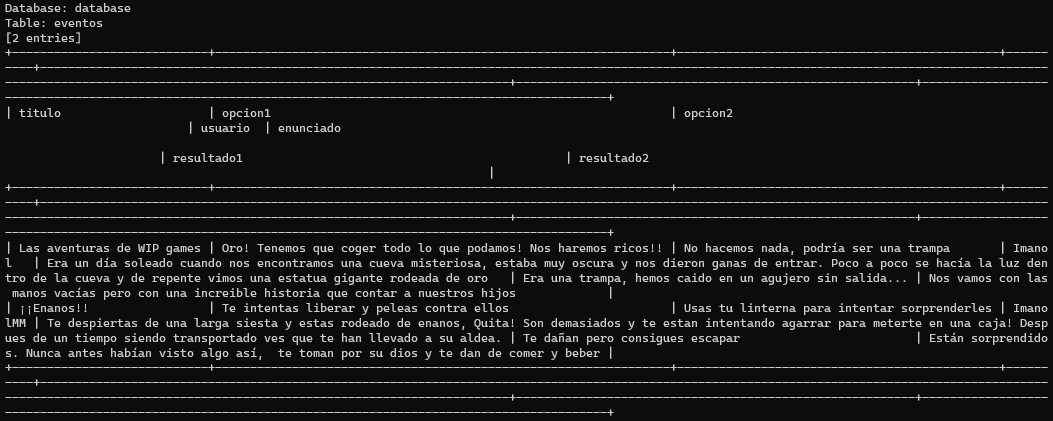
\includegraphics[width=1\textwidth]{./img/vulnerabilidades/2.3/1.3.png}
                    \caption{Tabla eventos de la base de datos}
                \end{figure}
                \clearpage
            \subsection{Cross Site Scripting}
                Tal y como hemos visto en la Introducción mediante el uso de ZAP hemos encontrado una vulnerabilidad de tipo XSS.
                En este caso, vamos a explotarlas de forma manual para ver que podemos hacer con ellas.
                Para ello accedemos al menu de 'Crear Evento' y en el campo 'Titulo' podemos introducir los siguientes codigos:
                \begin{enumerate}
                    \item \texttt{<script>alert("XSS")</script>}
                    \begin{itemize}
                        \item Este codigo nos muestra un mensaje de alerta con el texto 'XSS'
                        \begin{figure}[H]
                            \centering
                            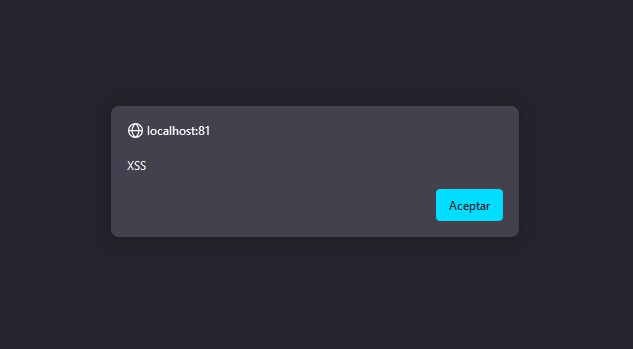
\includegraphics[width=1\textwidth]{./img/vulnerabilidades/2.3/2.1.png}
                            \caption{Alerta XSS}
                        \end{figure}
                    \end{itemize}
                    \item \texttt{<script>document.location="https://github.com/Xabierland"</script>}
                    \begin{itemize}
                        \item Este codigo nos redirige a mi pagina de Github
                    \end{itemize}
                    \item \texttt{<img src="https://shorturl.at/avFJO">}
                    \begin{itemize}
                        \item Este codigo nos muestra una imagen con el texto Pwned!
                        \begin{figure}[H]
                            \centering
                            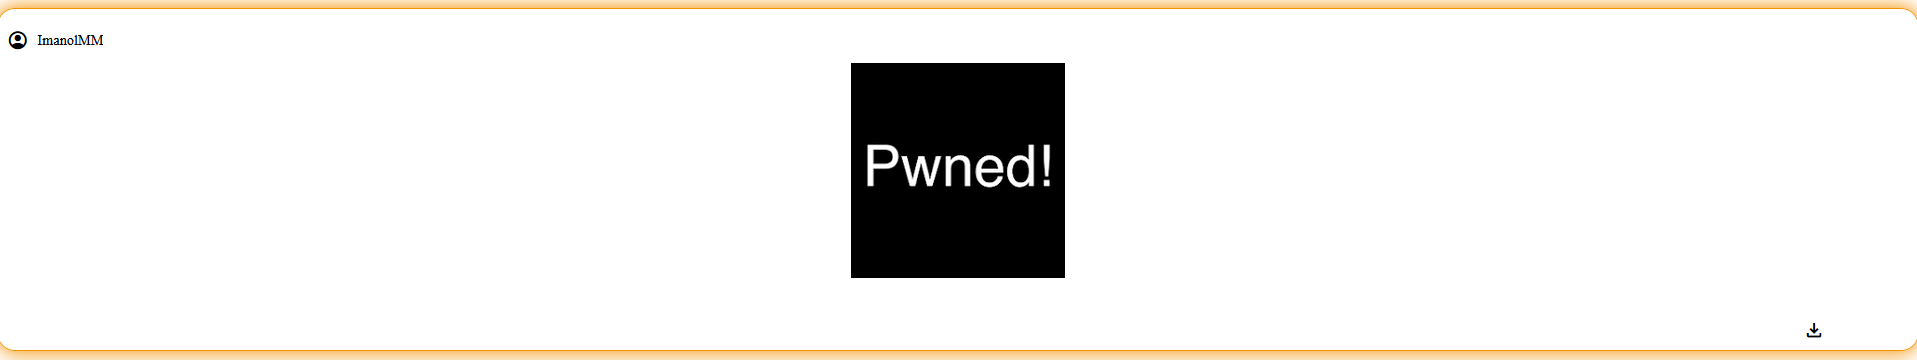
\includegraphics[width=1\textwidth]{./img/vulnerabilidades/2.3/2.3.png}
                            \caption{Imagen XSS}
                        \end{figure}
                    \end{itemize}
                    \item \texttt{<script>var paragraph = document.createElement('p');paragraph.textContent = 'Cookie: ' + document.cookie;document.body.appendChild(paragraph);</script>}
                    \begin{itemize}
                        \item Este codigo nos muestra el contenido de la cookie de php
                        \begin{figure}[H]
                            \centering
                            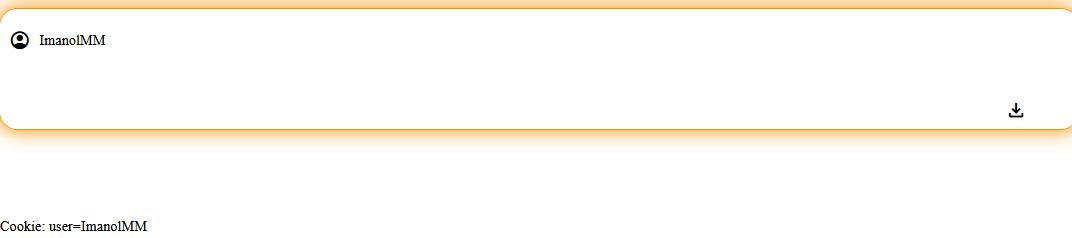
\includegraphics[width=1\textwidth]{./img/vulnerabilidades/2.3/2.4.png}
                            \caption{Cookie XSS}
                        \end{figure}
                    \end{itemize}
                \end{enumerate}
                Este tipo de vulnerabilidad es muy peligrosa ya que permite a un atacante ejecutar codigo en el navegador de la victima y realizar acciones en su nombre.\\

                Tambien hemos visto que podemos redirigir a la victima a una pagina maliciosa, lo que nos permitiria realizar un ataque de tipo Phishing.\\

                Aunque la carga de la imagen no parezca muy peligrosa, esta, en realidad puede darnos informacion como la IP de los usuarios que visitan la pagina ya que para cargar dicha imagen se realiza una peticion al servidor donde esta alojada dejando su IP en el camino.\\

                En este caso, hemos visto que podemos llegar incluso a ver la cookie de la victima, lo que nos permitiria hacer un ataque de tipo Session Hijacking.\\
                
                \clearpage
        \section{Configuración de seguridad insuficiente}
            \subsection{Fuga de información}
            \clearpage
            \subsection{Enumeración de directorios}
            \clearpage
            \subsection{Fuerza bruta}
            \clearpage
        \section{Componentes vulnerables y obsoletos}
            \subsection{Vulnerabilidades mediante MF}
            \clearpage
        \section{Fallos de identificación y autenticación}
            \subsection{Invalidación de sesiones}
            \clearpage
    \chapter{Bibliografia}
\end{document}